\PassOptionsToPackage{table,dvipsnames,svgnames}{xcolor}
\documentclass[portrait,final,a0paper]{nadiposter}

\usepackage{fontawesome}

\selectcolormodel{RGB}

\usepackage{graphicx}
\usepackage{multicol}
\usepackage{sectsty}

\usepackage{pgfbaselayers}
\pgfdeclarelayer{background}
\pgfdeclarelayer{foreground}
\pgfsetlayers{background,main,foreground}

\usepackage{amssymb}% http://ctan.org/pkg/amssymb
\usepackage{pifont}% http://ctan.org/pkg/pifont
\newcommand{\cmark}{\textcolor{blue}{\ding{51}}}%
\newcommand{\xmark}{\textcolor{red}{\ding{55}}}%
\newcommand{\pointer}{\scalebox{2}{\ding{43}}}%
% \usepackage{tikz}
% \def\checkmark{\tikz\fill[scale=0.4](0,.35) -- (.25,0) -- (1,.7) -- (.25,.15) -- cycle;}

\usepackage[backend=bibtex,style=numeric,maxnames=1, minnames=1]{biblatex}
\addbibresource{refs.bib}

%%%%%%%%%%%%%%%%%%%%%%%%%%%%%%%%%%%%%%%%%%%%%%%%%%%%%%%%%%%%%%%%%%%%%%%%%%%%%%%%
% Multicol Settings

\setlength{\columnsep}{1.5em}
\setlength{\columnseprule}{0mm}

%%%%%%%%%%%%%%%%%%%%%%%%%%%%%%%%%%%%%%%%%%%%%%%%%%%%%%%%%%%%%%%%%%%%%%%%%%%%%%%%


% ----------------------------------------------------------------------- %

% Useful hints
% https://tex.stackexchange.com/questions/252757/including-boxes-inside-boxes-in-baposter

% ----------------------------------------------------------------------- %



\newcommand{\compresslist}{%
\setlength{\itemsep}{1pt}%
\setlength{\parskip}{0pt}%
\setlength{\parsep}{0pt}%
\setlength{\leftmargin}{0pt}%
}


\contactInfo{%
\begin{tabular}{c}
  Viet Minh Vu and Beno\^it~Fr\'enay \\
  \faEnvelopeO\ : \{vuvietminh, benoit.frenay\}@unamur.be \\
\end{tabular}}



\begin{document}

\definecolor{unamurgreen}{RGB}{69,181,63}
\definecolor{unamurgray}{RGB}{64,68,67}
\definecolor{lightunamurgreen}{RGB}{69,181,63}

% from poster example

\definecolor{lightorange}{rgb}{0.9,0.4,0}
\definecolor{lightestorange}{rgb}{1,0.8,0.5}
\definecolor{darkorange}{rgb}{0.2,0.1,0}

% end from poster example


\typeout{Poster Starts}


\begin{poster}%
  % Poster Options
  {
  % Show grid to help with alignment
  % grid=true,
  grid=false,
  % Column spacing
  colspacing=1em,
  % Color style
  bgColorOne=lightunamurgreen,
  bgColorTwo=white,
  borderColor=unamurgray,
  headerColorOne=unamurgray,
  headerColorTwo=lightorange,
  headerFontColor=white,
  boxColorOne=white,
  boxColorTwo=white,
  % Format of textbox
  textborder=roundedright,
  % Format of text header
  eyecatcher=true,
  headerborder=closed,
  headerheight=0.1\textheight,
%  textfont=\sc, An example of changing the text font
  headershape=roundedleft,
  headershade=plain,
  headerfont=\Large\bf\textsc, %Sans Serif
  textfont={\setlength{\parindent}{1.5em}},
  boxshade=plain,
  background=plain,
  linewidth=2pt,
  columns=4
  }
  % Eye Catcher
  {\hbox{} } %
\includegraphics[height=7em]{images/nadi-red.png}} 
  % Title
  {\bf\textsc{Interactive Dimensionality Reduction Methods\\*[0.3em] for Visualization}\vspace{0.5em}}
  % Authors%   Viet~Minh~Vu,  Beno\^it~Fr\'enay
  {\textsc{Viet Minh Vu, Beno\^it~Fr\'enay} } % \\ {Universit\'e de Namur - Faculty of Computer Science}
  % University logo
  {% The makebox allows the title to flow into the logo, this is a hack because of the L shaped logo.
   \hbox{} % 
\includegraphics[height=7em]{images/nadi-red.png}
  }


% --------------------------------------------------------------------------- %

\sectionfont{\centering}

% --------------------------------------------------------------------------- %
\headerbox{Dimensionality Reduction (DR) methods in an Interactive Context}{name=interactiveDR,column=0,row=0,span=4}{

\begin{minipage}{0.63\linewidth}   
a
\end{minipage}
\begin{minipage}{0.33\linewidth}
b
\end{minipage}
}

% --------------------------------------------------------------------------- %
\headerbox{Different approaches for integrating user constraints}{name=constraint,column=0,span=4,below=interactiveDR}{
\begin{multicols}{2}
    \section*{\large{What are expressed by user (in high dim.)}}
    a
    \section*{\large{What are translated to the algorithm (in low dim.)}}
    b
\end{multicols}
}

% --------------------------------------------------------------------------- %
\headerbox{Proposed interactive t-SNE method}{name=method, column=0,span=4,below=constraint}{
a
}

% --------------------------------------------------------------------------- %
\headerbox{References}{name=ref,column=0,span=4,below=method}{
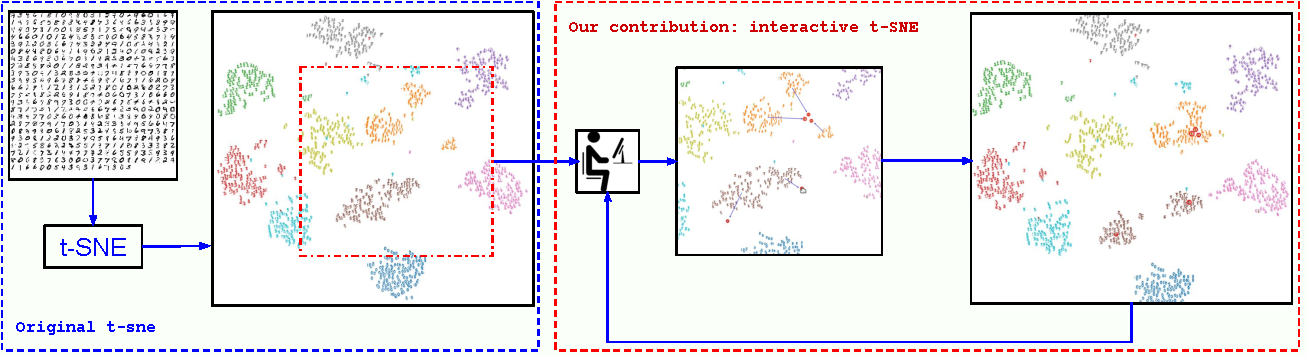
\includegraphics[width=0.9\linewidth]{poster_NADI_2018/images/tsnex.pdf}
}


\end{poster}

\end{document}

